\documentclass[10pt, conference, compsocconf]{IEEEtran}

%\usepackage{cite}
\usepackage[utf8]{inputenc}
\usepackage{graphicx}
\usepackage{epstopdf}
\usepackage{amsmath}
\usepackage{multirow}
\usepackage{lipsum}
\usepackage{caption}
\usepackage{subcaption}
\usepackage{setspace}
\usepackage{float}

\hyphenation{}

\renewcommand{\tablename}{Tabela}
\renewcommand{\figurename}{Figura}
\renewcommand{\refname}{Referências}

\begin{document}
\title{Estudo de dados de patologias cardíacas pediátricas}

\author{\IEEEauthorblockN{Filipe Figueiredo}
  \IEEEauthorblockA{201203559}
  \and
  \IEEEauthorblockN{Pedro Paredes}
  \IEEEauthorblockA{201205725}
}

\newcommand{\PreImg}[1]{
  \begin{figure}[H]
    \centering
    \includegraphics[scale=0.4]{img/pre_#1.png}
    \caption{Distribuição de {\tt #1} em relação a {\tt nxa}}
    \label{fig:pre#1}
  \end{figure}
}

\maketitle

% ----------------------------------------
% -                                      -
% ----------------------------------------

\section{Introdução}
\label{sec:int}

O uso de métodos estatísticos e computacionais para o estudo de dados
reais. Graças a evolução de métodos avançados de previsão e regressão,
uma área conhecida por ``Aprendizagem de Máquina'' (ou \textit{Machine
  Learning}), é possível estudar diversos problemas em diferentes
contextos. Esta análise é normalmente precedida de uma vasta análise
exploratória dos dados com diferentes fins, como a seleção de
atributos chave (por exemplo, através da determinação da correlações
entre os vários atributos) ou como a eliminação de \textit{outliers}
estatísticos.

Neste trabalho aplicamos várias destas técnicas comuns a um conjunto
de dados de patologias cardíacas de casos pediátricos. O objetivo
final é determinar quais variáveis têm maior ``poder'' de previsão
para determinar se um determinado sujeito possui alguma anormalidade
cardíaca e estudar o seu erro de classificação.

O resto deste relatório está organizado da seguinte forma. Na
Secção~\ref{sec:apr} descreve-se o \textit{dataset} usado assim como
os seus atributos e propriedades extrínsecas. Segue-se a descrição do
preprocessamento dos dados na Secção~\ref{sec:pre}, onde se indica as
correções base efetuadas por cada atributo e a devida
justificação. Posteriormente, na Secção~\ref{sec:ads} é feita uma
análise descritiva dos dados já processados, com o objetivo de se
estabelecer um perfil base dos dados. Na Secção~\ref{sec:afn} é feita
a análise final dos dados já processados, começando por verificar as
relações entre os pares de atributos e entre múltiplos atributos com
objetivo de efetuar uma escolha informada de atributos a usar para
aplicar algoritmos de classificação para determinar a presença de
anomalias cardíacas. Finalmente, na Secção~\ref{sec:cnd} são feitas
algumas notas finais e uma breve discussão das conclusões obtidas no
corpo do relatório.

% ----------------------------------------
% -                                      -
% ----------------------------------------

\section{Análise preliminar}
\label{sec:apr}

O \textit{dataset} fornecido para análise foi colecionado no Real
Hospital Português do Brasil, tendo sido posteriormente anonimizado e
enviado para Portugal com a autorização do Comité de ética do próprio
hospital. Os dados consistem em crianças entre os 0 e 19 anos, que
possuem ou não patologias cardíacas.

Na lista seguinte descrevemos em detalhe cada atributo presente nos
dados. A sigla de três letras indica o nome usado na análise dos dados
(presente na implementação que será descrita ao longo do relatório).

\begin{description}
  \item[\texttt{id}] Dado categórico que representa o número de identificação
    anonimizado do paciente
  \item[\texttt{pso}] Dado numérico contínuo que representa o peso do
    paciente em quilogramas
  \item[\texttt{alt}] Dado numérico contínuo que representa a altura
    do paciente em centímetros
  \item[\texttt{imc}] Dado numérico contínuo que representa o índice
    de massa corporal do paciente
  \item[\texttt{sex}] Dado categórico que representa o sexo do
    paciente
  \item[\texttt{atd}] Dado numérico discreto que representa a data em
    que o paciente foi atendido (e que os dados deste paciente foram
    colecionados)
  \item[\texttt{dn}] Dado numérico discreto que representa a data em
    que o paciente nasceu
  \item[\texttt{ide}] Dado numérico contínuo que representa a idade do
    paciente em anos
  \item[\texttt{cnv}] Dado categórico que representa a instituição de
    seguro de saúde a que pertence o paciente
  \item[\texttt{pls}] Dado categórico que representa o tipo de pulsos
    do paciente
  \item[\texttt{pas}] Dado numérico discreto que representa a pressão
    sistólica arterial do sangue do paciente em milímetros de mercúrio
  \item[\texttt{pad}] Dado numérico discreto que representa a pressão
    diastólica arterial do sangue do paciente em milímetros de mercúrio
  \item[\texttt{ppa}] Dado categórico que representa a relação entre a
    pressão sistólica e a diastólica do paciente
  \item[\texttt{b2}] Dado categórico que representa o segundo som
    cardíaco (ou o $S_2$) do paciente
  \item[\texttt{spr}] Dado categórico que representa o som cardíaco
    (sopro) do paciente
  \item[\texttt{fc}] Dado numérico discreto que representa a
    frequência de batimentos cardíacos do paciente
  \item[\texttt{hd1}] Dado categórico que representa o historial
    principal de doenças do paciente
  \item[\texttt{hd2}] Dado categórico que representa o historial
    secundário de doenças do paciente
  \item[\texttt{mo1}] Dado categórico que representa o motivo
    principal para admissão clínica do paciente
  \item[\texttt{mo2}] Dado categórico que representa o motivo
    secundário para admissão clínica do paciente
  \item[\texttt{nxa}] Dado categórico que representa a presença ou
    ausência de patologias cardíacas do paciente (atributo a prever)
\end{description}

Antes de se efetuar alguma análise aos dados, foi feita uma limpeza
simples dos dados. Primeiramente removemos as colunas de {\tt id} e
{\tt cnv}, pois são apenas administrativas e não serão úteis para
nenhuma análise. Além disso, renomeamos os atributos para as siglas de
3 letras usadas na descrição anterior, assim como os próprios valores
(por exemplo, no caso da variável {\tt nxa}, todas as entradas
passaram a ser do tipo ``nor'' ou ``ano'', representando
respetivamente, ``normal'' ou ausência de patologia e ``anormal'' ou
presença de patologia). De modo a facilitar a interpretação da
descrição de cada atributo, foram removidos elementos com mais de
$50\%$ de valores em falta. Finalmente foram tirados todos os valores
claramente incorretos, como idades negativas ou acima dos 20 anos,
datas posteriores à data atual \ldots

Tendo estas correções, passaremos a descrever cada atributo que se
manteve. Primeiramente, mostramos um sumário dos atributos numéricos
na Tabela~\ref{tab:nua}

\begin{table*}[!ht] \centering 
  \caption{Sumário dos atributos numéricos}
  \label{tab:nua} 
  \begin{tabular}{@{\extracolsep{5pt}}lccccccc} 
    \\[-1.8ex]\hline 
    \hline \\[-1.8ex] 
    Estatística & {\tt pso} & {\tt alt} & {\tt imc} & {\tt ide} & {\tt pas} & {\tt pad} & {\tt fc} \\ 
    \hline \\[-1.8ex] 
    N & 14,945 & 13,413 & 13,032 & 16,175 & 10,143 & 10,133 & 15,832 \\ 
    Média & 24.9 & 111.8 & 18.0 & 6.3 & 101.3 & 62.3 & 93.8 \\ 
    Desvio Padrão & 17.1 & 33.9 & 12.0 & 4.7 & 15.5 & 8.9 & 100.4 \\ 
    Mínimo & 0.3 & 10 & 5 & 0 & 10 & 6 & 8 \\ 
    Máximo & 157 & 198 & 848 & 19.8 & 990 & 120 & 9,288 \\ 
    {\tt NA}s & 2,928 & 4,460 & 4,841 & 1,698 & 7,730 & 7,740 & 2,041\\
    \hline \\[-1.8ex] 
  \end{tabular}
\end{table*}

Nas seguintes subseções iremos descrever cada um destes atributos em
detalhe, indicando a sua distribuição em relação a {\tt nxa} seguido
de uma breve discussão.

\subsection{\texttt{pso}}
Na Figura~\ref{fig:prepso} está representada a distribuição de valores
do atributo {\tt pso} em relação a {\tt nxa}.

\PreImg{pso}

A distribuição é influenciada pela variação de idades dos pacientes
considerados nos dados. Por esta razão, os dados aparentam ser
bimodais.

\subsection{\texttt{alt}}
Na Figura~\ref{fig:prealt} está representada a distribuição de valores
do atributo {\tt alt} em relação a {\tt nxa}.

\PreImg{alt}

A distribuição é semelhante à distribuição de {\tt pso} (com uma
escala diferente), o que já indica a possibilidade de uma correlação
entre os dois atributos. Adicionalmente, é também fortemente
influenciada pela idade.

\subsection{\texttt{imc}}
Na Figura~\ref{fig:preimc} está representada a distribuição de valores
do atributo {\tt imc} em relação a {\tt nxa}.

\PreImg{imc}

Este atributo é determinado unicamente a partir de {\tt pso} e {\tt
  alt}, o que é mostrado na sua distribuição. Porém, a influência da
idade é diminuída neste caso por ser a razão entre dois atributos com
influência semelhante.

\subsection{\texttt{sex}}
Na Figura~\ref{fig:presex} está representada a distribuição de valores
do atributo {\tt sex} em relação a {\tt nxa}.

\PreImg{sex}

Há uma ligeira tendência para elementos do sexo masculino, mas em
proporção aproximadamente equilibrada (cerca de $35\%$ para
$65\%$). Também é possível observar que a distribuição de {\tt nxa} em
cada um dos sexos é aproximadamente igual à distribuição marginal de
{\tt nxa}.

\subsection{\texttt{atd}}
Na Figura~\ref{fig:preatd} está representada a distribuição de valores
da variável {\tt atd}.

\begin{figure}[H]
  \centering
  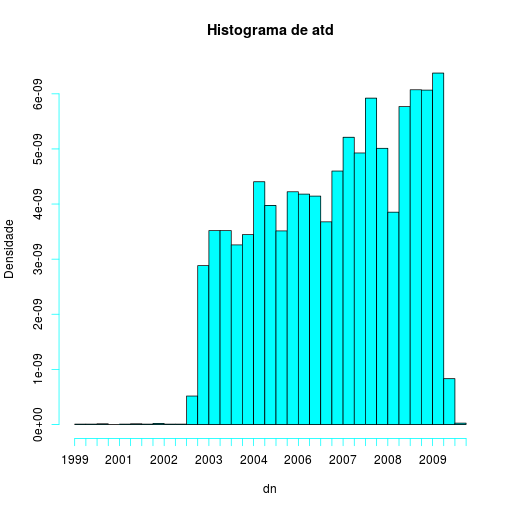
\includegraphics[scale=0.4]{img/pre_atd.png}
  \caption{Distribuição de {\tt atd}}
  \label{fig:preatd}
\end{figure}

\subsection{\texttt{dn}}
Na Figura~\ref{fig:predn} está representada a distribuição de valores
da variável {\tt dn} em relação à {\tt nxa}.

\PreImg{dn}

\subsection{\texttt{ide}}
Na Figura~\ref{fig:preide} está representada a distribuição de valores
da variável {\tt ide} em relação à {\tt nxa}.

\PreImg{ide}

\subsection{\texttt{pls}}
Na Figura~\ref{fig:prepls} está representada a distribuição de valores
da variável {\tt pls} em relação à {\tt nxa}.

\PreImg{pls}

\subsection{\texttt{pas}}
Na Figura~\ref{fig:prepas} está representada a distribuição de valores
da variável {\tt pas} em relação à {\tt nxa}.

\PreImg{pas}

\subsection{\texttt{pad}}
Na Figura~\ref{fig:prepad} está representada a distribuição de valores
da variável {\tt pad} em relação à {\tt nxa}.

\PreImg{pad}

\subsection{\texttt{ppa}}
Na Figura~\ref{fig:preppa} está representada a distribuição de valores
da variável {\tt ppa} em relação à {\tt nxa}.

\PreImg{ppa}

\subsection{\texttt{b2}}
Na Figura~\ref{fig:preb2} está representada a distribuição de valores
da variável {\tt b2} em relação à {\tt nxa}.

\PreImg{b2}

\subsection{\texttt{spr}}
Na Figura~\ref{fig:prespr} está representada a distribuição de valores
da variável {\tt spr} em relação à {\tt nxa}.

\PreImg{spr}

\subsection{\texttt{fc}}
Na Figura~\ref{fig:prefc} está representada a distribuição de valores
da variável {\tt fc} em relação à {\tt nxa}.

\PreImg{fc}

\subsection{\texttt{hd1}}
Na Figura~\ref{fig:prehd1} está representada a distribuição de valores
da variável {\tt hd1} em relação à {\tt nxa}.

\PreImg{hd1}

\subsection{\texttt{hd2}}
Na Figura~\ref{fig:prehd2} está representada a distribuição de valores
da variável {\tt hd2} em relação à {\tt nxa}.

\PreImg{hd2}

\subsection{\texttt{mo1}}
Na Figura~\ref{fig:premo1} está representada a distribuição de valores
da variável {\tt mo1} em relação à {\tt nxa}.

\PreImg{mo1}

\subsection{\texttt{mo2}}
Na Figura~\ref{fig:premo2} está representada a distribuição de valores
da variável {\tt mo2} em relação à {\tt nxa}.

\PreImg{mo2}

\subsection{\texttt{nxa}}
a

% ----------------------------------------
% -                                      -
% ----------------------------------------

\section{Preprocessamento de dados}
\label{sec:pre}

\lipsum[1]

% ----------------------------------------

\subsection{Transformação de dados}

\lipsum[2]

% ----------------------------------------

\subsection{Preenchimento de dados}

\lipsum[2]

% ----------------------------------------
% -                                      -
% ----------------------------------------

\section{Análise descritiva}
\label{sec:ads}

\lipsum[1]

\lipsum[2]

% ----------------------------------------
% -                                      -
% ----------------------------------------

\section{Análise final}
\label{sec:afn}

\lipsum[5]

% ----------------------------------------

\subsection{Análise bivariável}

\lipsum[2]

% ----------------------------------------

\subsection{Análise multivariável}

\lipsum[3]

% ----------------------------------------

\subsection{Análise de previsão}

\lipsum[4]

% ----------------------------------------

\subsubsection{Comparação de métodos}

\lipsum[5]

% ----------------------------------------
% -                                      -
% ----------------------------------------

\section{Conclusão e discussão}
\label{sec:cnd}

\lipsum[4]
\cite{boser1992training}

\small
\begin{spacing}{0.92}
\bibliographystyle{IEEEtran}
\bibliography{IEEEabrv,report}
\end{spacing}

\end{document}


